\documentclass[11pt]{article}

\usepackage[margin=1in]{geometry}
\usepackage{amsmath,amssymb,amsthm,mathtools}
\usepackage{bm}
\usepackage{enumitem}
\usepackage{xcolor}
\usepackage{microtype}
\usepackage{tikz}
\usepackage{hyperref}
\usepackage{fancyhdr}
\usepackage{booktabs}
\usepackage{array}

\hypersetup{hidelinks}
\setlength{\parindent}{0pt}
\setlength{\parskip}{0.55em}
\setlist[itemize]{leftmargin=1.55em,itemsep=0.2em,topsep=0.25em}
\setlist[enumerate]{leftmargin=1.7em,itemsep=0.2em,topsep=0.25em}

\pagestyle{fancy}
\fancyhf{}
\lhead{TV / BV / ROF Notes}
\rhead{}
\cfoot{\thepage}
\renewcommand{\headrulewidth}{0.3pt}

\newcommand{\Om}{\Omega}
\newcommand{\R}{\mathbb{R}}
\newcommand{\TV}{\operatorname{TV}}
\newcommand{\Div}{\operatorname{div}}
\newcommand{\supp}{\operatorname{supp}}
\newcommand{\esssup}{\operatorname*{ess\,sup}}
\newcommand{\avg}[1]{\overline{#1}_{\Om}}
\newcommand{\norm}[2][]{\left\lVert #2\right\rVert_{#1}}
\newcommand{\ip}[2]{\left\langle #1,#2\right\rangle}

\theoremstyle{definition}
\newtheorem{definition}{Definition}[section]
\newtheorem{example}[definition]{Example}
\newtheorem{remark}[definition]{Remark}
\theoremstyle{plain}
\newtheorem{theorem}[definition]{Theorem}
\newtheorem{lemma}[definition]{Lemma}
\newtheorem{proposition}[definition]{Proposition}

\title{\textbf{Total Variation Methods for Image Restoration}}
\author{}
\date{}

\begin{document}
\maketitle
\vspace{-1em}



\tableofcontents
\newpage

% ============================================================
\section{Functions of Bounded Variation and Total Variation}
% \textit{Source: ``Note Feb 14, 2022 TV Min'', pp. 1--4.}

Let $\Om\subset\R^2$ be open, bounded, and connected, with Lipschitz boundary. Let $f\in L^2(\Om)$ be given and let
\[
K:L^2(\Om)\to L^2(\Om)
\]
be linear and continuous. A model energy is
\[
F(u)=\lambda\int_{\Om}(Ku-f)^2\,dx+\int_{\Om}|\nabla u|\,dx,
\qquad \lambda>0.
\]
When $u$ is not differentiable in the classical sense, the second term is interpreted through total variation.

\subsection{From $W^{1,1}$ to $BV$}
In two dimensions,
\[
W^{1,1}(\Om)
=\left\{u\in L^1(\Om):\nabla u\in L^1(\Om)^2\right\}.
\]
Moreover,
\[
W^{1,1}(\Om)\subset L^2(\Om),
\]
so for $u\in W^{1,1}(\Om)$ the energy above is well-defined.

The norm
\[
\norm[W^{1,1}(\Om)]{u}
=\norm[L^1(\Om)]{u}+\norm[L^1(\Om)]{\nabla u}
\]
makes $W^{1,1}(\Om)$ a Banach space. However, $W^{1,1}$ is not reflexive, and limits of bounded sequences may develop jump discontinuities. This motivates the larger space $BV(\Om)$.

\begin{definition}[Total variation and $BV$]
For $u\in L^1(\Om)$, define
\[
\TV(u)
:=\sup\left\{
\int_{\Om}u\,\Div\varphi\,dx:
\varphi\in C_c^1(\Om;\R^2),\ \norm[L^\infty]{\varphi}\le 1
\right\}.
\]
We write
\[
\TV(u)=\int_{\Om}|Du|=\norm{Du}(\Om).
\]
Then
\[
BV(\Om):=\{u\in L^1(\Om):\TV(u)<\infty\}.
\]
\end{definition}

The notation $\int_{\Om}|Du|$ is used for the total variation measure. For smooth or Sobolev functions, it reduces to the usual gradient integral.

\begin{proposition}
If $u\in W^{1,1}(\Om)$, then $u\in BV(\Om)$ and
\[
\TV(u)=\int_{\Om}|\nabla u|\,dx.
\]
\end{proposition}

\begin{proof}
For $\varphi\in C_c^1(\Om;\R^2)$ with $\norm[L^\infty]{\varphi}\le1$, integration by parts gives
\[
\int_{\Om}u\,\Div\varphi\,dx
=-\int_{\Om}\nabla u\cdot\varphi\,dx
\le \int_{\Om}|\nabla u|\,dx.
\]
Hence $\TV(u)\le\int|\nabla u|$. Equality is obtained by approximating the pointwise direction $-\nabla u/|\nabla u|$ where $\nabla u\ne0$.
\end{proof}

Thus
\[
W^{1,1}(\Om)\subset BV(\Om).
\]
A standard norm on $BV$ is
\[
\norm[BV(\Om)]{u}
=\norm[L^1(\Om)]{u}+\norm{Du}(\Om).
\]

\subsection{Jump Discontinuities in $BV$}
Consider, on $(-1,1)$,
\[
u(x)=
\begin{cases}
-1,&-1\le x<0,\\
1,&0\le x\le1.
\end{cases}
\]
This $u$ is not in $W^{1,1}(-1,1)$, but it is in $BV(-1,1)$. Indeed, for $\phi\in C_c^1(-1,1)$,
\begin{align*}
\int_{-1}^1u\phi'\,dx
&=-\int_{-1}^0\phi'\,dx+\int_0^1\phi'\,dx\\
&=-[\phi(0)-\phi(-1)]+[\phi(1)-\phi(0)]\\
&=-2\phi(0),
\end{align*}
so
\[
\TV(u)=\sup_{\norm[L^\infty]{\phi}\le1}2|\phi(0)|=2.
\]

\begin{center}
\begin{tikzpicture}[scale=1.05]
\draw[->] (-2,0)--(2.2,0) node[right]{$x$};
\draw[->] (0,-1.5)--(0,1.5) node[above]{$u(x)$};
\draw[thick] (-1.7,-1)--(0,-1);
\draw[thick] (0,1)--(1.7,1);
\fill (0,1) circle (1.4pt);
\draw (0,-1) circle (1.4pt);
\node[left] at (0,1){$1$};
\node[right] at (0,-1){$-1$};
\end{tikzpicture}
\end{center}

\subsection{Convexity and Lower Semicontinuity}
\begin{proposition}[Convexity]
For $u,v\in BV(\Om)$ and $\theta\in[0,1]$,
\[
\norm{D(\theta u+(1-\theta)v)}(\Om)
\le \theta\norm{Du}(\Om)+(1-\theta)\norm{Dv}(\Om).
\]
\end{proposition}

\begin{proof}
Using the supremum definition,
\begin{align*}
\norm{D(\theta u+(1-\theta)v)}(\Om)
&=\sup_{\norm[L^\infty]{\varphi}\le1}
\int_{\Om}(\theta u+(1-\theta)v)\Div\varphi\,dx\\
&\le \theta\sup_{\varphi}\int_{\Om}u\Div\varphi\,dx
+(1-\theta)\sup_{\varphi}\int_{\Om}v\Div\varphi\,dx.
\end{align*}
\end{proof}

\begin{theorem}[Lower semicontinuity of total variation]
If $u_n\in BV(\Om)$ and $u_n\to u$ in $L^1(\Om)$, then
\[
\norm{Du}(\Om)\le \liminf_{n\to\infty}\norm{Du_n}(\Om).
\]
\end{theorem}

\begin{proof}
For every admissible $\varphi$,
\[
\int_{\Om}u\Div\varphi\,dx
=\lim_{n\to\infty}\int_{\Om}u_n\Div\varphi\,dx
\le \liminf_{n\to\infty}\norm{Du_n}(\Om).
\]
Taking the supremum over $\varphi$ yields the result.
\end{proof}

% ============================================================
\section{Compactness and Existence of Minimizers}
% \textit{Source: ``Note Feb 16--18, 2022 TV Min'', pp. 1--7.}

\begin{theorem}[Compactness in $BV$]
Suppose $u_n\in BV(\Om)$ and
\[
\norm[BV(\Om)]{u_n}\le C\qquad\text{for all }n.
\]
Then there is a subsequence $(u_{n_j})$ and $u\in BV(\Om)$ such that
\[
u_{n_j}\to u\quad\text{in }L^1(\Om),
\]
and
\[
\norm{Du}(\Om)
\le \liminf_{j\to\infty}\norm{Du_{n_j}}(\Om).
\]
\end{theorem}

\begin{theorem}[Generalized Poincar\'e--Wirtinger inequality in 2D]
Assume $\Om\subset\R^2$ is open, bounded, connected, with Lipschitz boundary. Then there exists $C=C(\Om)>0$ such that
\[
\norm[L^2(\Om)]{u-u_{\Om}}
\le C\norm{Du}(\Om),
\qquad u\in BV(\Om),
\]
where
\[
u_{\Om}:=\frac{1}{|\Om|}\int_{\Om}u(x)\,dx.
\]
In particular, in two dimensions $BV(\Om)\subset L^2(\Om)$.
\end{theorem}

\subsection{A General TV-Regularized Inverse Problem}
Assume
\[
K:L^2(\Om)\to L^2(\Om)
\]
is linear and continuous and
\[
K1_{\Om}\neq0.
\]
For $f\in L^2(\Om)$ and $\lambda>0$, define
\[
F(u)=\lambda\norm[L^2(\Om)]{Ku-f}^2+\norm{Du}(\Om),
\qquad u\in BV(\Om).
\]

\begin{theorem}[Existence]
The functional $F$ has at least one minimizer in $BV(\Om)$.
\end{theorem}

\begin{proof}
The functional is proper because, for example,
\[
F(0)=\lambda\norm[L^2]{f}^2<\infty.
\]
Take a minimizing sequence $(u_n)$ such that $F(u_n)\le M$. Then
\begin{align*}
\norm[L^2]{Ku_n-f}^2 &\le \frac{M}{\lambda},\\
\norm{Du_n}(\Om) &\le M.
\end{align*}

Write
\begin{align*}
v_n &= u_n-u_{n,\Om},\\
w_n &= u_{n,\Om},\\
u_n &= v_n+w_n,
\end{align*}
so that $v_{n,\Om}=0$. Since constants do not affect total variation,
\[
\norm{Dv_n}(\Om)=\norm{Du_n}(\Om)\le M.
\]
By Poincar\'e--Wirtinger,
\[
\norm[L^2]{v_n}\le C\norm{Dv_n}(\Om)\le C M.
\]
Also
\[
\norm[L^2]{K(v_n+w_n)-f}\le C_M.
\]
Since $K$ is bounded, $Kv_n$ is bounded. Therefore $Kw_n=w_nK1_{\Om}$ is bounded in $L^2$. Because $K1_{\Om}\neq0$, this controls the scalar $w_n$ and hence
\[
|u_{n,\Om}|=|w_n|\le C.
\]
Combining this with the bound on $v_n$ gives boundedness of $(u_n)$ in $L^2$, hence in $L^1$ because $\Om$ is bounded. Therefore $(u_n)$ is bounded in $BV(\Om)$.

By BV compactness, after passing to a subsequence,
\begin{align*}
u_{n_j} &\to u\quad\text{in }L^1(\Om),\\
\norm{Du}(\Om) &\le\liminf_j\norm{Du_{n_j}}(\Om).
\end{align*}
The same sequence is bounded in $L^2$, so after another subsequence it converges weakly in $L^2$ to the same $u$. Since $K$ is continuous linear,
\[
Ku_{n_j}\rightharpoonup Ku\quad\text{in }L^2.
\]
The squared $L^2$ norm is weakly lower semicontinuous, so
\[
\norm[L^2]{Ku-f}^2
\le\liminf_j\norm[L^2]{Ku_{n_j}-f}^2.
\]
Combining the two lower-semicontinuity inequalities yields
\[
F(u)\le\liminf_j F(u_{n_j})=\inf_{v\in BV(\Om)}F(v),
\]
so $u$ is a minimizer.
\end{proof}

\begin{theorem}[Uniqueness under injectivity]
If $K$ is injective, then the minimizer is unique.
\end{theorem}

\begin{proof}
The data-fidelity term $u\mapsto\norm{Ku-f}^2$ is strictly convex when $K$ is injective, while $u\mapsto\norm{Du}(\Om)$ is convex. Hence their sum is strictly convex.
\end{proof}

\subsection{Preservation of the Mean}
\begin{proposition}
Assume, in addition, that
\[
K1_{\Om}=1_{\Om}.
\]
If $u$ minimizes $F$, then
\[
\int_{\Om}Ku\,dx=\int_{\Om}f\,dx.
\]
\end{proposition}

\begin{proof}
For every constant $c\in\R$, minimality gives
\[
F(u)\le F(u+c).
\]
Since $D(u+c)=Du$, only the fidelity term changes. Thus $c=0$ minimizes
\[
H(c)=\norm[L^2]{K(u+c)-f}^2.
\]
Differentiating at $c=0$ gives
\[
0=H'(0)=2\int_{\Om}(Ku-f)(K1_{\Om})\,dx.
\]
Using $K1_{\Om}=1_{\Om}$ yields the claim.
\end{proof}

% ============================================================
\section{Constrained and Penalized Total Variation Models}
% \textit{Source: ``Note Feb 23--25, 2022 TV Min'', pp. 1--8.}

Assume for simplicity that $|\Om|=1$, that $BV(\Om)\subset L^2(\Om)$, and that
\[
K:L^2(\Om)\to L^2(\Om)
\]
is linear and continuous with $K1_{\Om}=1_{\Om}$. Let $f\in L^2(\Om)$ and let $\sigma>0$ denote the prescribed noise level.

Consider the following three related optimization problems.

\paragraph{Equality-constrained problem $(P_1)$.}
\[
(P_1)\qquad
\min_{u\in BV(\Om)}\norm{Du}(\Om)
\quad\text{subject to}\quad
\norm[L^2]{Ku-f}^2=\sigma^2.
\]
The equality constraint is not convex.

\paragraph{Inequality-constrained problem $(P_2)$.}
\[
(P_2)\qquad
\min_{u\in BV(\Om)}\norm{Du}(\Om)
\quad\text{subject to}\quad
\norm[L^2]{Ku-f}^2\le\sigma^2.
\]
This feasible set is convex.

\paragraph{Penalized problem $(P_3)$.}
\[
(P_3)_\lambda\qquad
\min_{u\in BV(\Om)}
\left\{
\norm{Du}(\Om)+\frac{\lambda}{2}\norm[L^2]{Ku-f}^2
\right\},
\qquad \lambda>0.
\]
This can be viewed as a Lagrange-multiplier formulation.

\subsection{Mean-Centered Formulation}
For $(P_1)$ it is enough to reduce to the case
\[
\int_{\Om}f(x)\,dx=0.
\]
Indeed, if $u$ solves $(P_1)$ for $f$, then
\[
\widetilde u=u-\int_{\Om}f(x)\,dx
\]
solves the corresponding problem for
\[
\widetilde f=f-\int_{\Om}f(x)\,dx,
\]
because $D\widetilde u=Du$ and $K1_{\Om}=1_{\Om}$.

\begin{lemma}[Mean identity at an equality-constrained minimizer]
If $u$ solves $(P_1)$, then
\[
\int_{\Om}Ku\,dx=\int_{\Om}f\,dx.
\]
\end{lemma}

\begin{proof}
As before, vary $u$ by a constant $c$. Since total variation does not change, $c=0$ minimizes
\[
\norm[L^2]{K(u+c)-f}^2.
\]
Differentiating at $c=0$ gives the identity.
\end{proof}

\subsection{Existence for the Equality-Constrained Problem}
Assume the feasible set is nonempty. Let $(u_n)$ be a minimizing sequence for $(P_1)$. The compactness argument from the previous section yields, after passing to a subsequence,
\begin{align*}
u_n &\to u\quad\text{in }L^1(\Om),\\
u_n &\rightharpoonup u\quad\text{in }L^2(\Om),
\end{align*}
and
\[
\norm{Du}(\Om)\le\liminf_n\norm{Du_n}(\Om).
\]
Weak lower semicontinuity gives
\[
\norm[L^2]{Ku-f}^2\le\sigma^2.
\]
If the inequality were strict, consider
\[
g(t)=\norm[L^2]{K(tu)-f}^2,
\qquad t\in[0,1].
\]
Under the mean-zero normalization, $g(0)=\norm{f}^2\ge\sigma^2$ while $g(1)<\sigma^2$. By continuity there is $\bar t\in[0,1)$ with $g(\bar t)=\sigma^2$. But
\[
\norm{D(\bar t u)}(\Om)=\bar t\norm{Du}(\Om)<\norm{Du}(\Om)
\]
unless the degenerate constant case occurs, contradicting minimality. Hence the equality constraint is recovered in the limit.

\subsection{Uniqueness for the Equality-Constrained Problem}
Suppose $u$ and $v$ are two solutions of $(P_1)$. Convexity gives
\[
\norm{D\left(\frac{u+v}{2}\right)}(\Om)
\le \frac12\norm{Du}(\Om)+\frac12\norm{Dv}(\Om).
\]
Also, by convexity of the squared norm,
\[
\norm[L^2]{K\left(\frac{u+v}{2}\right)-f}^2
\le \frac12\norm[L^2]{Ku-f}^2+
\frac12\norm[L^2]{Kv-f}^2
=\sigma^2.
\]
If the inequality is strict, scaling as above produces an admissible competitor with smaller total variation, impossible. Thus equality must hold in the strict-convexity inequality for the $L^2$ norm, so $Ku=Kv$. If $K$ is injective, $u=v$.

\subsection{Equivalence of Equality- and Inequality-Constrained Problems}
In the nondegenerate case, a minimizer of one constrained problem is a minimizer of the other. The key point is that a minimizer of $(P_2)$ cannot remain strictly inside the discrepancy ball unless it is the degenerate constant solution; otherwise scaling toward the boundary decreases total variation while preserving feasibility.

Equivalently,
\[
(P_1)\quad\Longleftrightarrow\quad(P_2)
\]
in the nondegenerate case.

\subsection{Gradient-Flow Formulation}
For a differentiable functional $F$, the formal gradient flow is
\begin{align*}
\frac{\partial u}{\partial t} &=-F'(u(t)),\\
u(0) &=u_0.
\end{align*}
Then
\[
\frac{d}{dt}F(u(t))
=F'(u(t))\frac{\partial u}{\partial t}
=-\left|\frac{\partial u}{\partial t}\right|^2\le0,
\]
so the energy decreases along the flow.

% ============================================================
\section{Discrepancy Analysis and Parameter Selection}
% \textit{Source: ``Note Feb 28, 2022 TV Min'', pp. 1--5.}

Let $u^\lambda$ solve
\[
(P_3)_\lambda:
\qquad
\min_{u\in BV(\Om)}
\left\{
\norm{Du}(\Om)+\frac{\lambda}{2}\norm[L^2]{Ku-f}^2
\right\}.
\]
Define the discrepancy
\[
\sigma(\lambda):=\norm[L^2]{Ku^\lambda-f}.
\]

\begin{proposition}[Monotonicity]
The function $\lambda\mapsto\sigma(\lambda)$ is non-increasing.
\end{proposition}

\begin{proof}
Let $\lambda>\mu\ge0$. Minimality gives
\begin{align*}
\norm{Du^\lambda}+\frac{\lambda}{2}\sigma(\lambda)^2
&\le \norm{Du^\mu}+\frac{\lambda}{2}\sigma(\mu)^2,\\
\norm{Du^\mu}+\frac{\mu}{2}\sigma(\mu)^2
&\le \norm{Du^\lambda}+\frac{\mu}{2}\sigma(\lambda)^2.
\end{align*}
Adding yields
\[
(\lambda-\mu)\bigl(\sigma(\lambda)^2-\sigma(\mu)^2\bigr)\le0.
\]
Thus $\sigma(\lambda)\le\sigma(\mu)$.
\end{proof}

If $\sigma(\lambda)=\sigma(\mu)$ for $\lambda<\mu$, then the two comparison inequalities force
\[
\norm{Du^\lambda}(\Om)=\norm{Du^\mu}(\Om),
\]
and the same function minimizes $(P_3)_{\lambda'}$ for every $\lambda'\in[\lambda,\mu]$.

Formally, a smooth minimizer satisfies
\[
-\Div\left(\frac{Du^\lambda}{|Du^\lambda|}\right)
+\lambda K^*(Ku^\lambda-f)=0
\quad\text{in }\Om,
\]
with natural boundary condition
\[
\frac{Du^\lambda}{|Du^\lambda|}\cdot n=0
\quad\text{on }\partial\Om.
\]
Testing by $u^\lambda$ gives
\[
\int_{\Om}|Du^\lambda|
=-\lambda\int_{\Om}(Ku^\lambda-f)\,Ku^\lambda\,dx.
\]
This identity explains why a flat portion of $\sigma(\lambda)$ can occur only near the degenerate constant regime. After a threshold $\bar\lambda$, the discrepancy is strictly decreasing, and
\[
\sigma(\lambda)\to0
\qquad\text{as }\lambda\to\infty
\]
in the well-posed setting.

\begin{center}
\begin{tikzpicture}[x=1.0cm,y=1.0cm]
\draw[->] (0,0)--(6.2,0) node[right]{$\lambda$};
\draw[->] (0,0)--(0,3.5) node[above]{$\sigma(\lambda)$};
\draw[thick] (0,2.8)--(1.6,2.8);
\draw[densely dotted] (1.6,0)--(1.6,2.8);
\draw[thick] plot[smooth] coordinates {(1.6,2.8)(2.1,2.15)(2.8,1.55)(3.8,0.95)(5.5,0.35)};
\node[below] at (1.6,0){$\bar\lambda$};
\end{tikzpicture}
\end{center}

\subsection{Iterative Parameter Selection}
To solve an equality-constrained problem with prescribed discrepancy $\sigma$, solve $(P_3)_\lambda$ repeatedly while adjusting $\lambda$.

Start with a small $\lambda>0$ and compute $u^\lambda$. If
\[
\sigma(\lambda)^2=\norm[L^2]{Ku^\lambda-f}^2>\sigma^2,
\]
increase $\lambda$; if the discrepancy is too small, decrease $\lambda$. One suggested update is
\[
\lambda\leftarrow
\max\left\{\lambda+\rho\bigl(\sigma(\lambda)^2-\sigma^2\bigr),0\right\},
\qquad \rho>0\ \text{small},
\]
and repeat until the discrepancy stabilizes at the desired level. The limiting $\lambda$ acts as the Lagrange multiplier for the equality constraint.

% ============================================================
\section{The Rudin--Osher--Fatemi Model}
% \textit{Source: ``Math273B-Lecture-ROF-TV-Part-I'', pp. 1--9.}

Let $\Om\subset\R^2$, often normalized so that $|\Om|=1$. The observed image is
\[
f\in L^2(\Om),
\]
and the unknown clean image is $u$. A linear degradation model is
\[
f=Ku+\eta,
\]
where $K$ is a bounded linear operator and $\eta$ is additive noise. Typical cases are
\begin{align*}
K &=I
\quad\text{(pure denoising)},\\
Ku &=k*u
\quad\text{(blur by convolution)}.
\end{align*}

The restoration problem is to recover $u$ from $f$, using knowledge of $K$ and statistical information about the noise.

\subsection{Variational Formulation of the ROF Model}
Rudin--Osher--Fatemi regularization uses total variation because it promotes smoothness while still allowing sharp edges. A clean image is often approximately piecewise smooth, with jump discontinuities along edges, so TV is more suitable than a quadratic $H^1$ penalty.

A constrained form is
\[
\min_u\int_{\Om}|\nabla u|\,dx
\quad\text{subject to}\quad
\int_{\Om}(Ku-f)^2\,dx=\sigma^2.
\]
The data-fidelity constraint reflects a noise model; for Gaussian noise, $\sigma^2$ represents a variance/energy level.

Introducing a Lagrange multiplier gives an unconstrained problem of the form
\[
\min_u\left\{
\int_{\Om}|\nabla u|\,dx
+\lambda\int_{\Om}(Ku-f)^2\,dx
\right\}.
\]
For $K=I$,
\[
\min_u\left\{
\int_{\Om}|\nabla u|\,dx
+\lambda\norm[L^2]{u-f}^2
\right\}.
\]
Here $\lambda$ tunes the balance:
\begin{itemize}
\item $\lambda$ large: the data term dominates, so $u\approx f$;
\item $\lambda$ small: the TV term dominates, producing a smoother, more nearly constant result;
\item in the limit $\lambda\downarrow0$ with $K=I$, the solution approaches the mean of $f$.
\end{itemize}

\subsection{Ill-Posedness and Regularization}
Without the TV term, inversion of $K$ may be unstable or impossible: $K$ can be non-invertible, and even when formally invertible its inverse may amplify noise. The regularizer stabilizes the inverse problem.

\subsection{Formal Euler--Lagrange Equations}
For comparison, if the regularizer were quadratic,
\[
\int_{\Om}|\nabla u|^2\,dx,
\]
then the corresponding Euler--Lagrange equation would contain a Laplacian. With the TV regularizer, formally
\[
\frac{\partial}{\partial \nabla u}|\nabla u|
=\frac{\nabla u}{|\nabla u|}.
\]
For
\[
F(u)=\int_{\Om}|\nabla u|\,dx
+\lambda\norm[L^2]{Ku-f}^2,
\]
the formal first-order condition is
\[
2\lambda K^*(Ku-f)
-\Div\left(\frac{\nabla u}{|\nabla u|}\right)=0
\quad\text{in }\Om,
\]
with natural boundary condition
\[
\frac{\nabla u}{|\nabla u|}\cdot n=0
\quad\text{on }\partial\Om.
\]
For a convolution operator $Ku=k*u$, the adjoint is convolution with the reflected kernel $k^*$; in Fourier variables the formal least-squares inverse involves division by $|\widehat{k}|^2$, which explains the instability when $\widehat{k}$ is small.

\subsection{Geometric Interpretation of Total Variation}
At a regular point of a level set of $u$,
\[
N=\frac{\nabla u}{|\nabla u|}
\]
is normal to the level set. The term
\[
\Div\left(\frac{\nabla u}{|\nabla u|}\right)
\]
is the curvature of the level set (up to sign convention). Thus the TV Euler--Lagrange equation smooths mainly in the normal/curvature geometry while preserving sharp interfaces better than isotropic quadratic diffusion.

\begin{center}
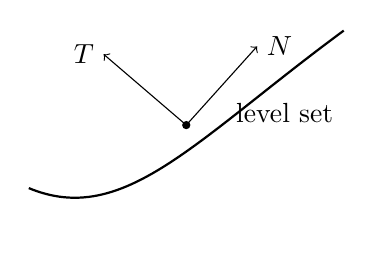
\begin{tikzpicture}[scale=1]
\draw[thick] (-2,-0.8) .. controls (-0.8,-1.3) and (0.1,-0.2) .. (2,1.2);
\fill (0,0) circle (1.5pt);
\draw[->] (0,0)--(0.9,1.0) node[right]{$N$};
\draw[->] (0,0)--(-1.05,0.9) node[left]{$T$};
\node at (1.25,0.15){level set};
\end{tikzpicture}
\end{center}

% ============================================================
\section{Relationships Between Constrained and Penalized ROF Models}
% \textit{Source: ``Math273B-Lecture-ROF-TV-Part-II'', pp. 1--9.}

The two central problems are
\[
(P_1)\qquad
\min_u \TV(u)
\quad\text{subject to}\quad
\norm[L^2]{Ku-f}^2=\sigma^2,
\]
and
\[
(P_2)_\lambda\qquad
\min_u\left\{
\TV(u)+\frac{\lambda}{2}\norm[L^2]{Ku-f}^2
\right\},
\qquad \lambda>0.
\]
For a solution $u^\lambda$ of $(P_2)_\lambda$, define
\[
\sigma(\lambda)=\norm[L^2]{Ku^\lambda-f}.
\]
As shown earlier, $\sigma(\lambda)$ is non-increasing.

The discrepancy exhibits the following qualitative behavior:
\begin{itemize}
\item for very small $\lambda$, the solution can remain constant and $\sigma(\lambda)$ may have an initial plateau;
\item after a threshold $\bar\lambda$, the discrepancy decreases strictly;
\item $\sigma(\lambda)\to0$ as $\lambda\to\infty$ under the stated assumptions.
\end{itemize}
Thus, to realize a prescribed discrepancy $\sigma$, one can tune $\lambda$ until
\[
\norm[L^2]{Ku^\lambda-f}^2\approx\sigma^2.
\]

\subsection{A Gradient-Flow Construction for the Constrained Problem}
For clarity, take $K=I$. Consider
\[
(P_1)\qquad
\min_u\int_{\Om}|\nabla u|\,dx
\quad\text{subject to}\quad
\int_{\Om}(f-u)^2\,dx=\sigma^2.
\]
The Lagrangian gradient flow is formally
\[
\frac{\partial u}{\partial t}
=2\lambda(t)(f-u)
+\Div\left(\frac{\nabla u}{|\nabla u|}\right),
\qquad t>0.
\]
Choose $u(0)=u^0$ so that
\[
\int_{\Om}(f-u^0)^2\,dx=\sigma^2,
\]
and impose preservation of the constraint:
\[
\frac{d}{dt}\int_{\Om}(f-u(t))^2\,dx=0.
\]
Substituting the flow equation yields
\[
\lambda(t)
=-\frac{
\displaystyle\int_{\Om}(f-u(t))
\Div\left(\frac{\nabla u(t)}{|\nabla u(t)|}\right)\,dx
}{
\displaystyle 2\int_{\Om}(f-u(t))^2\,dx
}.
\]
After integration by parts and using the natural boundary condition,
\[
\lambda(t)=
\frac{
\displaystyle\int_{\Om}\nabla f\cdot\frac{\nabla u(t)}{|\nabla u(t)|}\,dx
-\displaystyle\int_{\Om}|\nabla u(t)|\,dx
}{
\displaystyle 2\int_{\Om}(f-u(t))^2\,dx
}
\]
which gives the multiplier update for the constrained flow.

% ============================================================
\section{Chambolle's Projection Algorithm}
% \textit{Source: ``Math273B-Lecture-Chambolle-ProjAlg'', pp. 1--8.}

For denoising, take $K=I$ and consider the ROF proximal problem
\begin{align*}
&\min_{u\in L^2(\Om)}
\left\{
\frac{1}{2\lambda}\norm[L^2]{u-f}^2+J(u)
\right\},\\
&J(u)=\TV(u),\quad \lambda>0.
\end{align*}
Here $f$ is the given noisy image and $u$ is the restored image.

Three computational approaches are:
\begin{enumerate}
\item solve the Euler--Lagrange equation by finite differences;
\item discretize the functional and apply an optimization method;
\item use Chambolle's projection algorithm, which works through a dual/projection formulation.
\end{enumerate}

\subsection{Convex Analysis Preliminaries}
For a proper convex lower-semicontinuous functional $G$, the following convex-analytic principles apply:
\begin{itemize}
\item subgradient duality:
\[
 u^*\in\partial G(u)
 \quad\Longleftrightarrow\quad
 u\in\partial G^*(u^*);
\]
\item Fenchel--Moreau:
\[
G^{**}=G;
\]
\item proximity maps as projections when the conjugate is an indicator of a convex set.
\end{itemize}

\subsection{The Polar Representation of TV}
Let
\[
V=L^2(\Om)^2
\]
and define the indicator functional
\[
G(p)=
\begin{cases}
0,& |p(x)|\le1\ \text{a.e.},\\
+\infty,&\text{otherwise}.
\end{cases}
\]
Then
\[
C:=\{p\in L^2(\Om)^2:|p(x)|\le1\ \text{a.e.}\}
\]
is convex and closed. Its Fenchel conjugate is
\[
G^*(p^*)
=\sup_{p\in C}\int_{\Om}p^*\cdot p\,dx
=\int_{\Om}|p^*|\,dx.
\]
Thus the $L^1$ norm of a vector field is the support function of the pointwise unit ball.

Now take the linear operator $\Lambda=\nabla$. Formally $\Lambda^*=-\Div$. Therefore
\[
J(u)=\int_{\Om}|\nabla u|\,dx
=\sup_{|p|\le1}\int_{\Om}\nabla u\cdot p\,dx
=\sup_{|p|\le1}\int_{\Om}u(-\Div p)\,dx,
\]
up to the chosen boundary/sign convention.

It is convenient to introduce the closed convex polar set
\[
\widetilde C
:=\{\Div p:\ p\in L^2(\Om)^2,\ |p(x)|\le1\ \text{a.e.}\}.
\]
With the sign convention used here, the polar of $J$ is represented by $\widetilde C$.

\subsection{Proximal Point as an Orthogonal Projection}
A minimizer $u$ satisfies
\[
0\in u-f+\lambda\,\partial J(u).
\]
Equivalently,
\[
\frac{f-u}{\lambda}\in\partial J(u)
\quad\Longleftrightarrow\quad
u\in\partial J^*\left(\frac{f-u}{\lambda}\right).
\]
Let
\[
w:=\frac{f-u}{\lambda}.
\]
Then $w$ is the minimizer of
\[
\frac12\norm[L^2]{w-f/\lambda}^2+\frac{1}{\lambda}J^*(w).
\]
Since $J^*$ is the indicator of $\widetilde C$,
\[
 w=P_{\widetilde C}\left(\frac{f}{\lambda}\right)
\]
and therefore
\[
 u=f-\lambda w.
\]
Thus TV denoising is reduced to a projection problem.

Since $w=\Div p$ for some vector field $p=(p_1,p_2)$ with $|p(x)|\le1$, the projection can be written as
\[
\min_{|p(x)|\le1}
\left\|
\frac{f}{\lambda}-\Div p
\right\|_{L^2(\Om)}^2.
\]

\subsection{Euler--Lagrange/KKT Form of the Dual Problem}
Introduce a pointwise Lagrange multiplier $\alpha(x)\ge0$ for the constraint $|p(x)|^2\le1$. The Lagrangian has the form
\[
\left\|\frac{f}{\lambda}-\Div p\right\|_2^2
+\int_{\Om}\alpha(x)(|p(x)|^2-1)\,dx.
\]
The formal stationarity condition is
\[
\nabla\left(\frac{f}{\lambda}-\Div p\right)+\alpha(x)p(x)=0.
\]
If $|p(x)|<1$, the constraint is inactive and $\alpha(x)=0$. If $|p(x)|=1$, then
\[
\alpha(x)p(x)
=-\nabla\left(\frac{f}{\lambda}-\Div p\right),
\]
so
\[
\alpha(x)=
\left|\nabla\left(\frac{f}{\lambda}-\Div p\right)\right|.
\]
Both cases are therefore covered by
\[
\alpha(x)=
\left|\nabla\left(\frac{f}{\lambda}-\Div p\right)\right|.
\]

This leads to a projected/fixed-point iteration for $p$. In the standard discrete form,
\[
 p^{n+1}
 =\frac{
 p^n+\tau\,\nabla\left(\Div p^n-f/\lambda\right)
 }{
 1+\tau\left|\nabla\left(\Div p^n-f/\lambda\right)\right|
 }
\]
(pointwise in the image grid), starting from $p^0$ with $\norm[L^\infty]{p^0}\le1$. After convergence,
\[
u=f-\lambda\Div p.
\]



\subsection{Computational Advantages of the Dual Formulation}
The primal and dual formulations have different computational properties:
\begin{itemize}
\item the primal variable $u$ contains the linear, non-differentiable TV term $J(u)=\int|\nabla u|$, so direct gradient methods can converge slowly and need a regularization such as
\[
\int_{\Om}|\nabla u|\,dx
\approx
\int_{\Om}\sqrt{\varepsilon^2+|\nabla u|^2}\,dx,
\qquad \varepsilon\downarrow0;
\]
\item the dual/projection problem is quadratic in $p$ with a simple pointwise unit-ball constraint, making it better suited to efficient iterations.
\end{itemize}

% ============================================================
\end{document}
